\chapter[Gyda's Saucy Message]{
    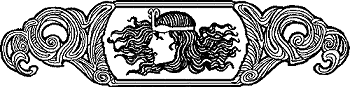
\includegraphics[width=9.3cm]{viking-tales/026}\\
    Gyda's Saucy Message}

\lettrine{N}{ow} Harald heard men talk of Gyda, the daughter of King
Eric.
\vskip2\baselineskip
``She is very beautiful,'' they said, ``but she is very proud, too. She
can both read and make runes. No other woman in the world knows so much
about herbs as she does. She can cure any sickness. And she is proud of
all this!''

Now when King Harald heard that, he thought to himself:

``Fair and proud. I like them both. I will have her for my wife.''

So he called his uncle, Guthorm, and said:

``Take rich gifts and go to Gyda's foster-father\footnote{See note about
foster-father on page~\pageref{foster-father}.} and tell him that I will
marry Gyda.''

So Guthorm and his men came to that house and they told the king's
message to the foster-father. Gyda was standing near, weaving a rich
cloak. She heard the speech. She came up and said, holding her head high
and curling her lip:

``I will not waste myself on a king of so few people. Norway is a
strange country. There is a little king here and a little king
there--hundreds of them scattered about. Now in Denmark there is but one
great king over the whole land. And it is so in Sweden. Is no one brave
enough to make all of Norway his own?''

She laughed a scornful laugh and walked away. The men stood with open
mouths and stared after her. Could it be that she had sent that saucy
message to King Harald? They looked at her foster-father. He was
chuckling in his beard and said nothing to them. They started out of the
house in anger. When they were at the door, Gyda came up to them again
and said:

``Give this message to your King Harald for me: I will not be his wife
unless he puts all of Norway under him for my sake.''

\begin{figure}[ht]
    \centering
    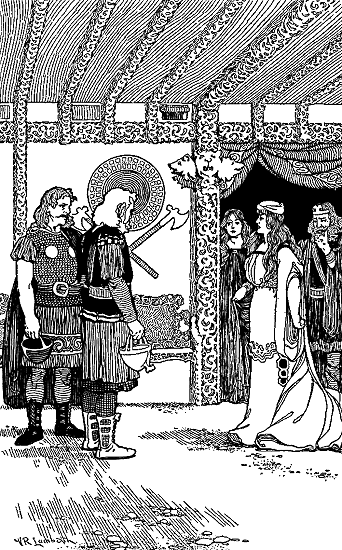
\includegraphics[width=9.1cm]{viking-tales/027}
    \caption{``I will not be his wife unless he puts all of Norway under
        him for my sake''}
\end{figure}

So Guthorm and his men rode homeward across the country. They did not
talk. They were all thinking. At last one said:

``How shall we give this message to the king?''

``I have been thinking of that,'' Guthorm said; ``his anger is no little
thing.''

It was late when they rode into the king's yard; for they had ridden
slowly, trying to make some plan for softening the message, but they had
thought of none.

``I see light through the wind's-eyes of the feast hall,'' one said.

``Yes, the king keeps feast,'' Guthorm said. ``We must give our message
before all his guests.''

So they went in with very heavy hearts. There sat King Harald in the
high seat. The benches on both sides were full of men. The tables had
been taken out, and the mead-horns were going round.

``Oh, ho!'' cried King Harald. ``Our messengers! What news?''

Then Guthorm said:

``This Gyda is a bold and saucy girl, King Harald. My tongue refuses to
give her message.''

The king stamped his foot.

``Out with it!'' he cried. ``What does she say?''

``She says that she will not marry so little a king,'' Guthorm answered.

Harald jumped to his feet. His face flushed red. Guthorm stretched out
his hand.

``They are not my words, O King; they are the words of a silly girl.''

``Is there any more?'' the king shouted. ``Go on!''

``She said: `There is one king in Denmark and one king in Sweden. Is
there no man brave enough to make himself king of all Norway? Tell King
Harald that I will not marry him unless he puts all of Norway under him
for my sake.'''

The guests sat speechless, staring at Guthorm. All at once the king
broke into a roar of laughter.

``By the hammer of Thor!'' he cried, ``that is a good message. I thank
you, Gyda. Did you hear it, friends? King of all Norway! Why, we are all
stupids. Why did we not think of that?''

Then he raised his horn high.

``Now hear my vow. I say that I will not cut my hair or comb it until I
am king of all Norway. That I will be or I will die.''

Then he drank off the horn of mead, and while he drank it, all the men
in the hall stood up and waved their swords and shouted and shouted.
That old hall in all its two hundred years of feasts had not heard such
a noise before.

``Ah, Harald!'' Guthorm cried, ``surely Thor in Valhalla smiled when he
heard that vow.''

The men sat all night talking of that wonderful vow.

On the very next day King Harald sent out his war-arrows. Soon a great
army was gathered. They marched through the country north and south and
east and west, burning houses and fighting battles as they went. People
fled before them, some to their own kings, some inland to the deep woods
and hid there. But some went to King Harald and said:

``We will be your men.''

``Then take the oath, and I will be friends with you,'' he said.

The men took off their swords and laid them down and came one by one and
knelt before the king. They put their heads between his knees and said:

``From this day, Harald Halfdanson, I am your man. I will serve you in
war. For my land I will pay you taxes. I will be faithful to you as my
king.''

Then Harald said:

``I am your king, and I will be faithful to you.''

Many kings took that oath and thousands of common men. Of all the
battles that Harald fought, he did not lose one.

Now for a long time the king's hair and beard had not been combed or
cut. They stood out around his head in a great bushy mat of yellow. At a
feast one day when the jokes were going round, Harald's uncle said:

``Harald, I will give you a new name. After this you shall be called
Harald Shockhead. As my naming gift I give you this drinking-horn.''

``It is a good name,'' laughed all the men.

After that all people called him Harald Shockhead.

During these wars, whenever King Harald got a country for his own, this
is what he did. He said:

``All the marshland and the woodland where no people live is mine. For
his farm every man shall pay me taxes.''

Over every country he put some brave, wise man and called him Earl. He
said to the earls:

``You shall collect the taxes and pay them to me. But some you shall
keep for yourselves. You shall punish any man who steals or murders or
does any wicked thing. When your people are in trouble they shall come
to you, and you shall set the thing right. You must keep peace in the
land. I will not have my people troubled with robber vikings.''

The earls did all these things as best they could; for they were good
strong men. The farmers were happy. They said:

``We can work on our farms with peace now. Before King Harald came,
something was always wrong. The vikings would come and steal our gold
and our grain and burn our houses, or the king would call us to war.
Those little kings are always fighting. It is better under King
Harald.''

But the chiefs, who liked to fight and go a-viking, hated King Harald
and his new ways. One of these chiefs was Solfi. He was a king's son.
Harald had killed his father in battle. Solfi had been in that battle.
At the end of it he fled away with two hundred men and got into ships.

``We will make that Shockhead smart,'' he said.

So they harried the coast of King Harald's country. They filled their
ships with gold. They ate other men's meals. They burned farmhouses
behind them. The people cried out to the earls for help. So the earls
had out their ships all the time trying to catch Solfi, but he was too
clever for them.

In the spring he went to a certain king, Audbiorn, and said to him:

``Now, there are two things that we can do. We can become this Shockhead
Harald's thralls, we can kneel before him and put our heads between his
knees. Or else we can fight. My father thought it better to die in
battle than to be any man's thrall. How is it? Will you join with my
cousin Arnvid and me against this young Shockhead?''

``Yes, I will do it,'' said the king.

\begin{figure}[hb]
    \centering
    \vskip8pt
    
\includegraphics[width=2.7cm]{viking-tales/011}
\end{figure}
